

El consensus contiene las dinámicas de los agentes y es posible conocer la evolución de las trayectorias, pero estos valore son ideales. La implementación de dicho algoritmo en un sistema real deberá tener en cuenta las dinámicas propias de cada agente. En este escenario los valores resultado del consensus serán los valores de referencia para los agentes(actuadores) como se observa en la Figura \ref{fig_consensus_piston}. El sistema real debe ser estable y llegar a un valor de referencia dado. Por ejemplo para nuestro caso el actuador es un pistón hidráulico con un controlador proporcional integral que sigue un valor de referencia.

\begin{figure}[!h]
\centering
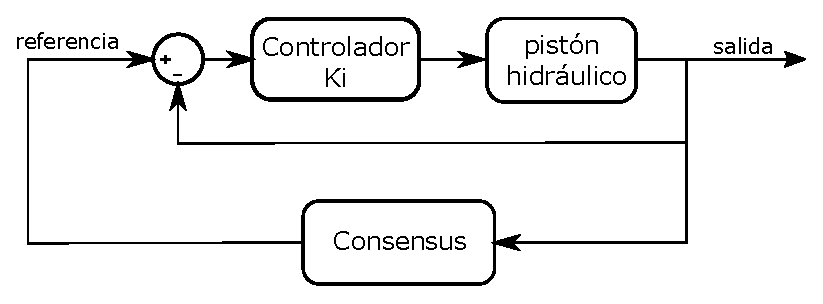
\includegraphics[width=3in]{imagenes/consensus_piston.eps}
\caption{Esquema de conexión Consensus-Planta}
\label{fig_consensus_piston}
\end{figure}

Las dinámicas de cambio del consensus idealmente deben ser más lentas que las del sistema físico con el objetivo de que la planta pueda seguir la trayectoria trazada por el consensus. Para efectos prácticos de la implementación desde el punto de vista discreto el periodo del consensus deberá ser mayor que el de la planta. Para que exista una mejor interacción consensus-planta, el valor de entrada para cada iteración del consensus será el valor de posición de la planta (ver Figura \ref{fig_consensus_piston}), esto conlleva a que si los actuadores son lentos, el consensus "espere" a la planta, pero si la planta es sufucientemente rápida la planta no influirá en el comportamiento del consensus.

